\section{Métricas usadas para evaluar el rendimiento de las técnicas de filtrado}
\label{sec:metrics}

Usualmente, para evaluar el desempeño de un algoritmo de filtrado de ruido en señales de habla se utilizan dos tipos de evaluaciones; la evaluación objetiva y la evaluación subjetiva.

La evaluación objetiva, consiste en utilizar técnicas de procesamiento de señales para comparar qué tan diferentes son la señal original sin ruido, con la señal filtrada generada como salida del algoritmo en evaluación.

Por otro lado, la evaluación subjetiva consiste en realizar un ensayo donde se tiene un grupo de oyentes los cuales califican el grado de supresión de los ruidos presentes en la señal de habla.

En la práctica resulta más eficiente la utilización de una evaluación objetiva, ya que reduce los tiempos de ejecución, los costos y la complejidad de la tarea en general. Para que la evaluación objetiva resulte efectiva es imperioso la utilización de métricas que tengan una alta correlación con los resultados de la evaluación subjetiva.

\subsection{Calidad vs Inteligibilidad}
\label{sec:intelligibility_vs_quality}

Dos de los atributos usualmente evaluados para medir la eficacia de un algoritmo de supresión de ruido en señales de habla son; la calidad y la inteligibilidad de las señales resultantes.

La calidad hace referencia a características de la señal tales como natural, rasposa, ronca, áspera, robótica, etc.

La inteligibilidad hace referencia a la identificación del contenido. Una señal de habla tiene alta inteligibilidad si los fonemas y las palabras presentes en ella se pueden identificar correctamente.

Ambas métricas tienen cierto grado de correlación pero hay casos donde se tiene alta inteligibilidad y baja calidad. Por ejemplo, una señal de habla sintetizada con una baja cantidad de armónicos, donde usualmente la señal es percibida como robótica pero los fonemas y palabras se pueden identificar correctamente \cite{philipos_book_speech_enhancement}. 

\subsection{Calidad}

Usualmente, las métricas objetivas de calidad de la señal de habla son implementadas primero segmentando la señal en ventanas de 10 a 30 ms y luego computando una medida de distorsión entre la señal original y la señal procesada. Luego, la calidad global se computa promediando las calidades individuales de cada ventana.

Actualmente la métrica mas utilizada para evaluar la calidad de un algoritmo de filtrado de ruidos en señales de habla es la denominada Medida de evaluación perceptiva de la calidad del habla \cite{perceptual_evaluation_of_speech_quality_a_new_method_for_speech_quality_assessment_of_telephone_networks_and_codecs,speech_enhancement_theory_and_practice} (PESQ por sus siglas en ingles).

A diferencia de otras medidas de calidad, la PESQ está diseñada para tener en cuenta distorsiones comúnmente encontradas en aplicaciones del mundo real, donde las señales son transmitidas por distintos canales y codificadas de distintas formas.  Algunas de estas distorsiones son: ruido de fondo, pérdida de paquetes, retardos variables, efectos de filtrado y distorsión por codificación.

La PESQ fue desarrollada en una competición creada por la Unión Internacional de Telecomunicaciones (ITU-T) con el objetivo de encontrar una métrica objetiva que tenga alto grado de correlación con las observaciones subjetivas reportadas ante las condiciones antes descritas. La PESQ se convirtió en la métrica recomendada por la ITU-T para la evaluación de la calidad de una señal de habla.

El diagrama en bloques de la PESQ lo podemos ver en la figura \ref{fig:ch4_pesq_schematic}. A continuación se detalla el objetivo de cada bloque.

\begin{figure}
	\centering
	\centerline{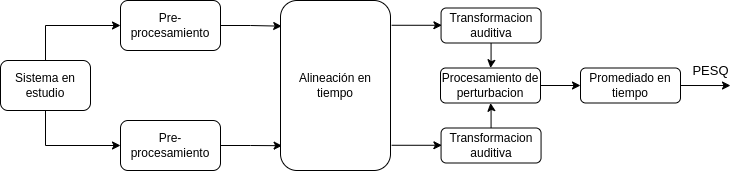
\includegraphics[scale=0.6]{images/ch4/pesq_schematic.png}}
	\caption{Diagrama en bloques de la medida PESQ. Figura tomada de \cite{speech_enhancement_theory_and_practice}.}
	\label{fig:ch4_pesq_schematic}
\end{figure}

\subsubsection{Pre-procesamiento}

La primera etapa de la PESQ tiene dos funciones. La primera es nivelar la señal de habla ruidosa y la señal procesada a un nivel estándar de audición. Las compensaciones a aplicar a cada señal se obtienen por tramos utilizando el valor RMS luego de ser filtradas por un filtro pasa-banda cuyas frecuencias de corte inferior y superior tienen un valor de 350 y 3250 Hz respectivamente.

La segunda etapa es un filtro cuya respuesta en frecuencia es similar a la respuesta en frecuencia típica de un micrófono de teléfono.

\subsubsection{Alineación}

Para poder realizar una comparación adecuada entre la señal de habla sin ruido y la señal filtrada, es necesario que éstas estén alineadas en el dominio del tiempo. Por esta razón la PESQ incorpora un proceso de alineación de ambas señales.

El proceso de alineación consta de dos pasos; primero se divide la señal en secciones de 64 ms y luego, para cada sección, se obtiene la correlación cruzada entre ambas señales. El máximo valor obtenido durante la correlación provee una estimación del retraso entre ambas señales en esa sección.

\subsubsection{Transformación auditiva}

El nivel de sonoridad percibido por el oído humano no es lineal en función de la frecuencia sino que es logarítmico, la sensación sonora de intensidad, es decir la sonoridad, se agudiza para sonidos débiles, y disminuye para sonidos fuertes. Para tener en cuenta este factor, la medida PESQ incorpora un bloque de transformación auditiva que transforma las señales en una representación de la sonoridad percibida por el oído humano.

El primer paso del bloque de transformación auditiva es obtener una estimación del espectro de potencia. La obtención se hace por medio de computar la FFT, utilizando una ventana de Hamming de 32 ms con un solapamiento del 50\%. Luego se computa el espectro basado en la escala Bark \cite{analytical_expressions_for_critical_band_rate_and_critical_bandwidth_as_a_function_of_frequency} por medio de sumar las potencias en 42 bandas.

El segundo paso del bloque de transformación auditiva es transformar el espectro de potencia a una medida de sonoridad utilizando el modelo de Zwicker \cite{a_revision_of_zwicker_s_loudness_model}.

\subsubsection{Cómputo de la perturbación}

La densidad de perturbación se obtiene como:

\begin{equation*}
	r_n(b) = S_n(b) - \bar{S}_n(b)
\end{equation*}

\noindent donde:

\begin{itemize}
	\item $S_n(b)$ es el resultado de pasar la señal original por el bloque de transformación auditiva.
	\item $\bar{S}_n(b)$ es el resultado de pasar la señal procesada por el bloque de transformación auditiva.
\end{itemize}

A la densidad de perturbación se la usa como una medida de error audible y se la utiliza para el cómputo final de la medida PESQ.

En la densidad de perturbación, para cada banda de frecuencias, habrá diferencias positivas y diferencias negativas. Una diferencia positiva, es decir $S_n(b) > \bar{S}_n(b)$, indica que un componente como el ruido se ha sumado a la señal original, mientras que una diferencia negativa, es decir $S_n(b) < \bar{S}_n(b)$, indica que un componente espectral ha sido omitido. Un componente omitido, a diferencia de un componente aditivo, no afecta en gran medida la calidad percibida, debido a los efectos de enmascaramiento. Por lo tanto, las diferencias positivas tienen más peso en el cómputo final de la PESQ que las diferencias negativas.

Una vez sopesadas las diferencias negativas y positivas se integra en frecuencia la densidad de perturbación para obtener el valor final de perturbación de cada segmento.

El valor final de la medida PESQ se obtiene promediando los valores de perturbación obtenidos para cada segmento. El rango de la medida PESQ varía entre $-0.5$ y $4.5$.

\subsection{Inteligibilidad}

Como vimos en la sección \ref{sec:intelligibility_vs_quality}, una señal de habla tiene alta inteligibilidad si los fonemas y las palabras en ella se pueden identificar correctamente.

La mayoría de las métricas de inteligibilidad se basan en la hipótesis de que ésta depende de qué tan audible sea la señal en cada banda de frecuencia. Una señal será audible en aquellas bandas de frecuencia donde la SNR es positiva. A medida que la SNR se acerque a 0 o se vuelva negativa, la señal comenzará a ser inaudible y por lo tanto la inteligibilidad tenderá a disminuir.  

El problema que tienen este tipo de métricas es que no son adecuadas para evaluar la variación de la inteligibilidad generada por filtros que utilizan ganancias variables en tiempo y frecuencia para suprimir el ruido presente en las señales de habla \cite{an_algorithm_for_intelligibility_prediction_of_time_frequency_weighted_noisy_speech}. 

En \cite{an_algorithm_for_intelligibility_prediction_of_time_frequency_weighted_noisy_speech} buscaron definir una métrica de inteligibilidad que tenga alto grado de correlación con las evaluaciones subjetivas realizadas a filtros que utilizan ganancias variables en tiempo y frecuencia. A la métrica en cuestión la nombraron Medida de inteligibilidad objetiva de corto plazo (STOI por sus siglas en inglés).

El diagrama en bloques de la STOI lo podemos ver en la figura \ref{fig:ch4_stoi_schematic}. A continuación se detalla el proceso completo para obtener la medida STOI.

\begin{figure}
	\centering
	\centerline{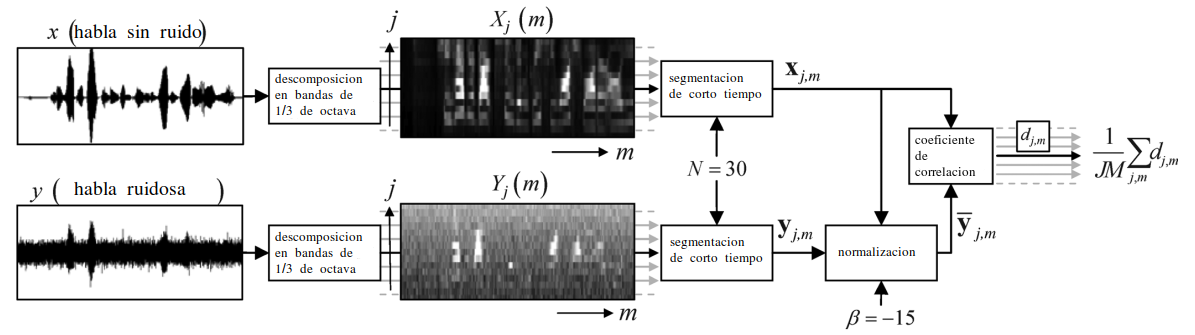
\includegraphics[scale=0.4]{images/ch4/stoi_schematic.png}}
	\caption{Diagrama en bloques de la medida STOI. Figura tomada de \cite{an_algorithm_for_intelligibility_prediction_of_time_frequency_weighted_noisy_speech}.}
	\label{fig:ch4_stoi_schematic}
\end{figure}

\subsubsection{Descomposición en bandas de 1/3 de octava}

El primer paso de la STOI es descomponer, tanto la señal original como la señal procesada en tiempo y frecuencia. Para ello se aplica la STFT utilizando una ventana de Hann de 256 muestras con un solapamiento del 50\%. A cada uno de los segmentos se lo completa con 0 para que alcance un tamaño de 512 muestras.

\subsubsection{Remoción de regiones de no-habla}

El segundo paso es remover las regiones de no-habla, ya que no contribuyen a la medida de inteligibilidad. Por definición la inteligibilidad depende de qué tan distinguibles sean las palabras.

Para remover las regiones de no-habla se realizan los siguientes pasos:

\begin{enumerate}
	\item Se busca la ventana con mayor energía en la señal original sin ruido.
	\item Se buscan todas las ventanas de la señal original cuyo valor de energía sea $\SI{40}{dB}$ menor al máximo encontrado en (1).
	\item Se remueven todas las ventanas encontradas en (2) tanto de la señal original como de la señal procesada.
\end{enumerate}

\subsubsection{Cálculo de la unidad TF}

El tercer paso es agrupar las frecuencias en bandas de 1/3 de octava. Se usan un total de 15 bandas, donde la frecuencia central de la banda más chica es 150 Hz y la de la banda más grande es de 4.3 kHz. 

La medida STOI define la unidad TF de la señal original como:

\begin{equation*}
	X_j(m) = \sqrt{\sum_{k=k_1(j)}^{k_2(j) - 1} | \hat{x}(k,m) |^2}
\end{equation*}

donde:

\begin{itemize}
	\item $j$ es el índice de la banda de 1/3 de octava.
	\item $\hat{x}(k,m)$ es la muestra $k$ de la DFT de la ventana $m$ de la señal $x$.
	\item $k_1$ es el límite inferior de la banda de 1/3 de octava.
	\item $k_2$ es el límite superior de la banda de 1/3 de octava.
\end{itemize}

La unidad TF de la señal procesada se define de igual manera y se la denota como $Y_j(m)$. Por último, se definen los vectores $x_{j,m}$ y $y_{j,m}$ como:

\begin{align*}
	x_{j,m} &= [X_j(m - N + 1), X_j(m - N + 2), ..., X_j(m)]^T \\ \\
	y_{j,m} &= [Y_j(m - N + 1), Y_j(m - N + 2), ..., Y_j(m)]^T
\end{align*}

\subsubsection{Cálculo de la STOI}

La medida intermedia de inteligibilidad se calcula como el coeficiente de correlación muestral entre los vectores $x_{j,m}$ y $y_{j,m}$:

\begin{equation*}
	d_{j,m} = \frac{(x_{j,m} - \mu_{x_{j,m}})^T (y_{j,m} - \mu_{y_{j,m}})}{|| x_{j,m} - \mu_{x_{j,m}} || \; ||y_{j,m} - \mu_{y_{j,m}}||}
\end{equation*}

donde $\mu_{x_{j,m}}$ es la media muestral del vector $x_{j,m}$ y $\mu_{y_{j,m}}$ es la media muestral del vector $y_{j,m}$.

Finalmente la STOI se define como:

\begin{equation*}
	d = \frac{1}{JM} \sum_{j,m} d_{j,m}
\end{equation*}

donde $M$ es la cantidad total de ventanas y $J$ la cantidad de bandas de 1/3 de octava. El rango de la medida STOI varía entre $0$ y $1$.